% 2003 年粤桂卷第 21 题：矩形动点与交点轨迹示意图
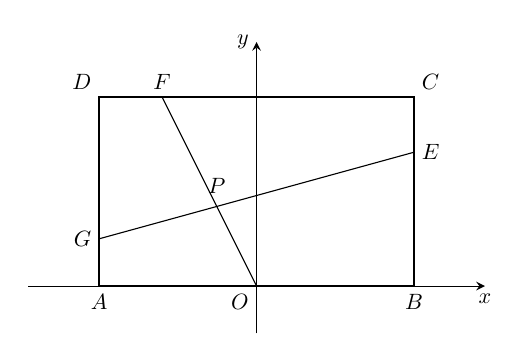
\begin{tikzpicture}[>=stealth,scale=1.0]
  % 矩形顶点与原点
  \coordinate (A) at (-2, 0);
  \coordinate (B) at (2, 0);
  \coordinate (O) at (0, 0);
  \coordinate (C) at (2, 2.4);
  \coordinate (D) at (-2, 2.4);

  % 坐标轴
  \draw[->] (-2.9, 0) -- (2.9, 0) node[below,scale=0.8] {$x$};
  \draw[->] (0, -0.6) -- (0, 3.1) node[left,scale=0.8] {$y$};

  % 矩形 ABCD
  \draw[thick] (A) -- (B) -- (C) -- (D) -- cycle;

  % 动点 E, F, G
  \coordinate (F) at (-1.2, 2.4);
  \coordinate (G) at (-2, 0.6);
  \coordinate (E) at (2, 1.7);

  % 线段 GE 与 OF
  \draw (G) -- (E);
  \draw (O) -- (F);

  % 交点 P
  \coordinate (P) at (intersection of G--E and O--F);

  % 顶点与动点标注
  \node[below,scale=0.8] at (A) {$A$};
  \node[below,scale=0.8] at (B) {$B$};
  \node[below left,scale=0.8] at (O) {$O$};
  \node[above right,scale=0.8] at (C) {$C$};
  \node[above left,scale=0.8] at (D) {$D$};
  \node[right,scale=0.8] at (E) {$E$};
  \node[above,scale=0.8] at (F) {$F$};
  \node[left,scale=0.8] at (G) {$G$};
  \node[above=2pt,scale=0.8] at (P) {$P$};
\end{tikzpicture}
